\subsection{Ca sử dụng xem thông tin chi tiết địa điểm du lịch}
\vspace{0.5cm}


\noindent 
\begin{tabularx}{\linewidth}{| l | X |} 
\hline 
\textbf{Mô tả} & Người dùng xem chi tiết thông tin địa điểm du lịch.  \\ 
\hline 
\textbf{Luồng cơ bản} & 1. Người dùng bấm vào một địa điểm du lịch muốn xem thông tin\newline
                
                        2. Hệ thống hiển thị thông tin chi tiết địa điểm du lịch. \\
                        vị trí hiện tại. \\
                     
% \hline 
% \textbf{Luồng thay thế} & Người dùng không cấp quyền truy cập vị trí sẽ nhận thông báo lỗi.\\           
\hline 
\textbf{Tiền điều kiện} & Người dùng đang đăng nhập và phiên đăng nhập chưa kết thúc. \\
\hline 
\textbf{Hậu điều kiện} &- Người dùng có thể xem thông tin về địa điểm như mô tả, địa chỉ, sđt, ảnh. \newline
                        - Người dùng có thể xem chi tiết các đánh giá về địa điểm. \newline
                        - Người dùng có thể xem chi tiết các địa điểm liên quan. \\

\hline 
\textbf{Yêu cầu phi chức năng} & Hệ thống xử lý lấy thông tin không quá 2s  \\ 
\hline 
\end{tabularx}

\vspace{0.8cm}

\noindent 
\begin{tabular}{| c | c |}
    \hline
    \textbf{Biểu đồ hoạt động} & \textbf{Quan hệ} \\ 
    \hline
    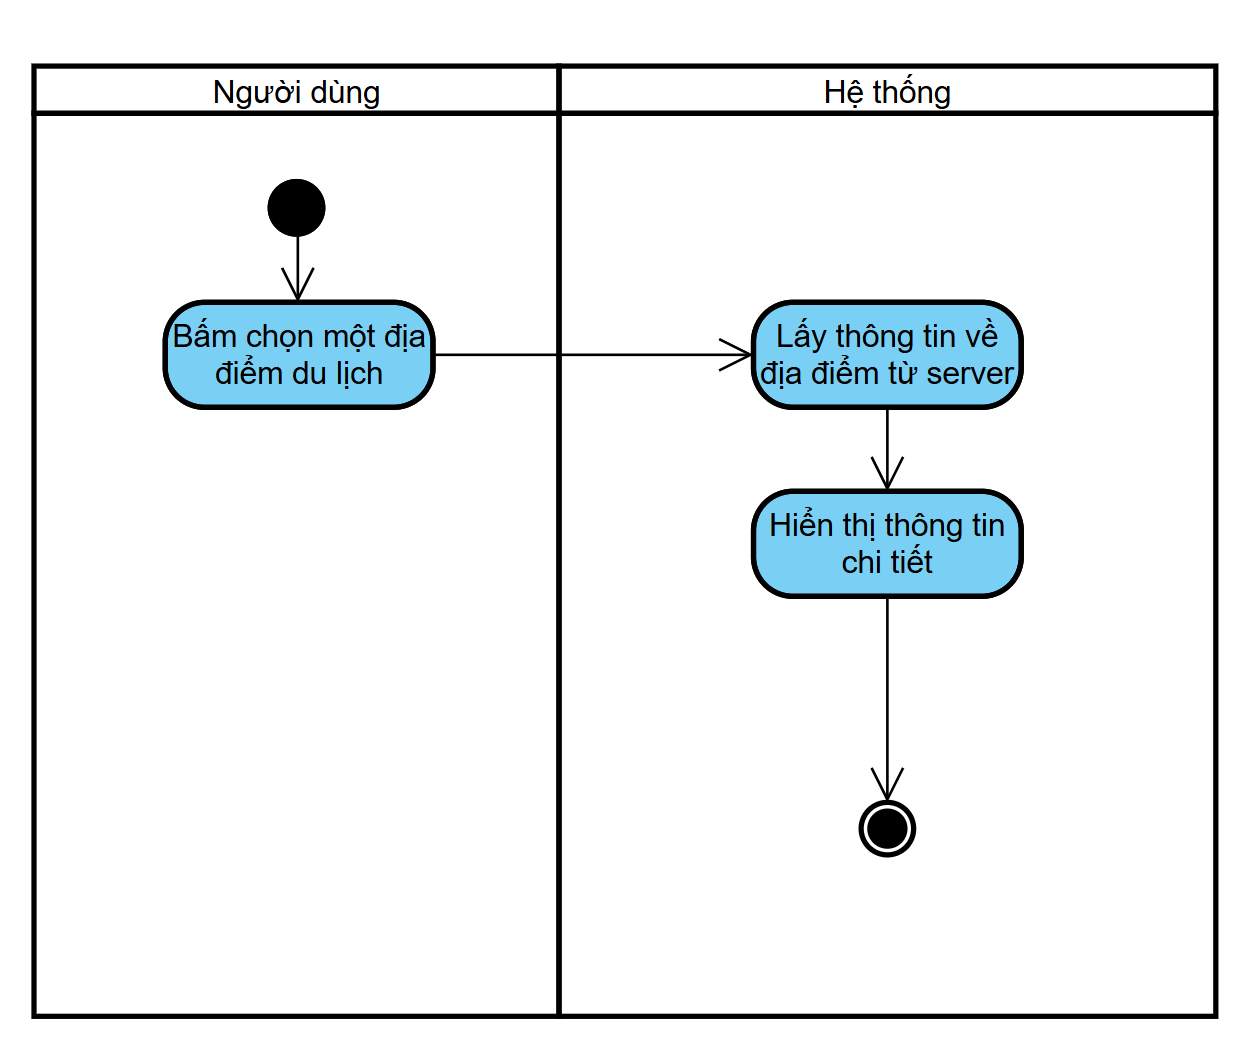
\includegraphics[width=0.5\linewidth]{figures/c3/3-3-8-ad.png} 
    & 
    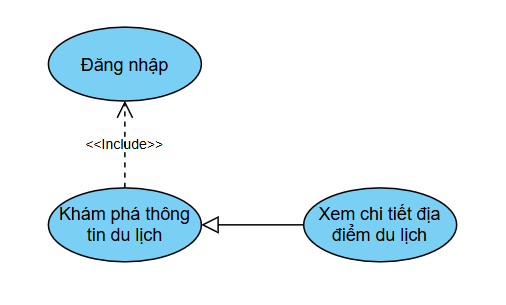
\includegraphics[width=0.45\linewidth]{figures/c3/3-3-8-rd.png} \\ 
    \hline
\end{tabular}


\vspace{0.8cm}

\begin{figure}[H]
    \centering  
    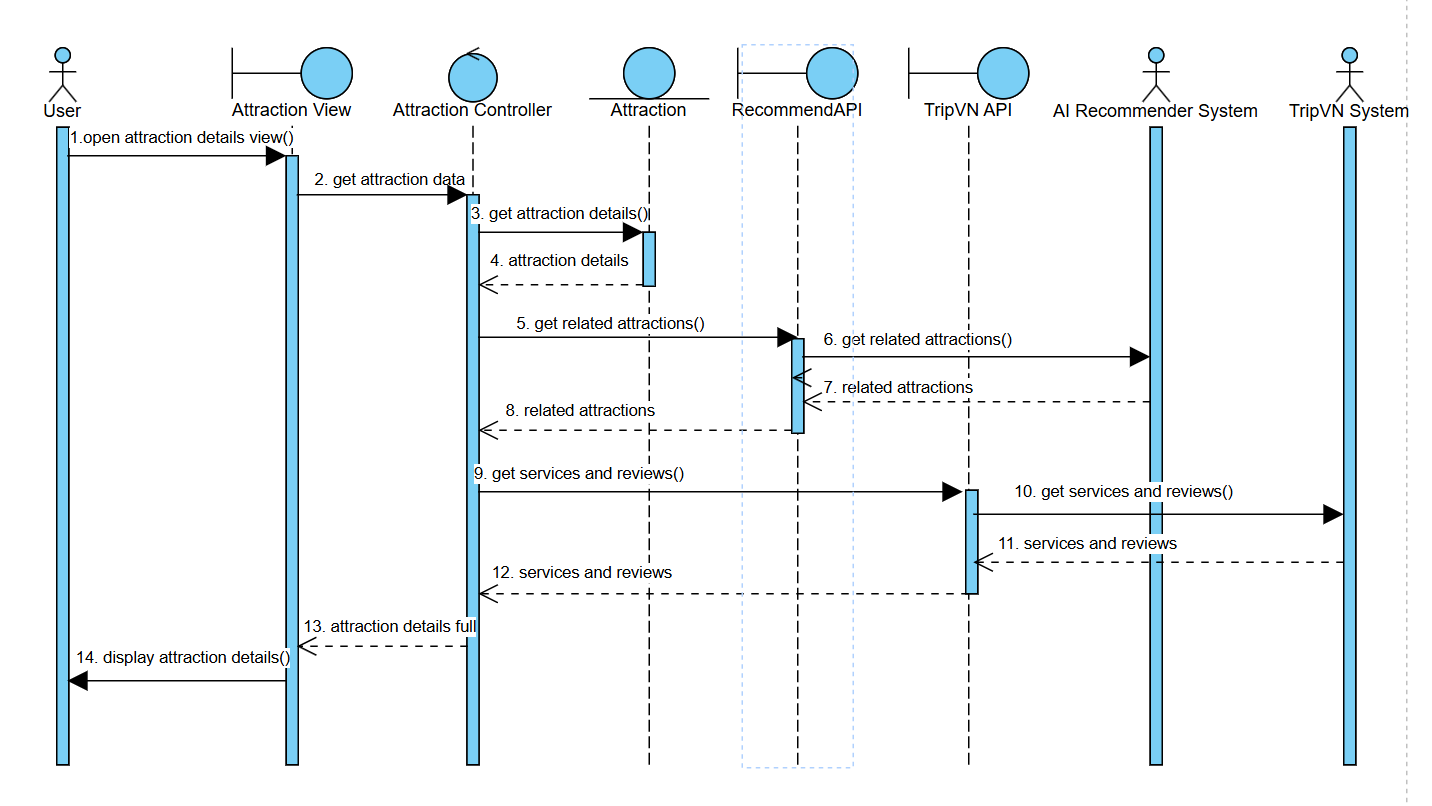
\includegraphics[width=1\textwidth]{figures/c3/3-3-8-sd.png}
    \caption{Biểu đồ tuần tự ca sử dụng xem thông tin chi tiết địa điểm du lịch.}
    \label{fig:3-3-8-sequence-diagram}
\end{figure}